\documentclass{book}

\usepackage{amssymb}
\usepackage{amsmath}
\usepackage{amsthm}
\usepackage{arydshln}
\usepackage{calc}
\usepackage{cancel}
\usepackage{caption}
\usepackage{cite}
\usepackage{color}
\usepackage{enumitem}
\usepackage{esint}
\usepackage{etoolbox}
\usepackage{float}
\usepackage{framed}
\usepackage{fullpage}
\usepackage{gensymb}
\usepackage[margin=1in]{geometry}
\usepackage{graphicx}
\usepackage{listings}
\usepackage{multirow}
\usepackage{subfiles}
\usepackage{rsfso}
\usepackage{tikz}
\usepackage{tikz-3dplot}
\usepackage{ushort}
\usepackage{wrapfig}
\usepackage{xcolor}
\usepackage{soul}
\usepackage{epstopdf}

% pdf versions
\pdfoptionpdfminorversion=7

% handle page stretching
\raggedbottom

% Graphics file location
\graphicspath{{Graphics/}{../Graphics/}}

% Use for drawings
\usetikzlibrary{angles,arrows,calc,decorations,intersections,patterns,positioning,quotes,shapes}
\usetikzlibrary{shapes.geometric}
\usetikzlibrary{decorations.pathreplacing}
\newcommand{\midarrow}{\tikz \draw[-latex] (0,0) -- +(.1,0);}

% Tikz commands for drawing block diagrams, etc...
\tikzset{%
	block/.style    = {draw, rectangle, minimum height = 2em, minimum width = 2em},
	sum/.style      = {draw, circle}, % Adder
	input/.style    = {fill=white, rectangle}, % Input
	output/.style   = {fill=white, rectangle}, % Output
	waypoint/.style   = {coordinate}, % Output
}

\tikzset{%
	startstop/.style= {draw, rectangle, rounded corners, minimum width=2cm, minimum height=1cm,text centered},
	inout/.style    = {draw, trapezium, trapezium left angle=70, trapezium right angle=110, minimum width=2cm, minimum height=1cm, text centered},
	process/.style  = {draw, rectangle, minimum width=2cm, minimum height=1cm, text centered},
	decision/.style = {draw, diamond, minimum width=1.5cm, minimum height=1cm, text centered, diamond, aspect=2},
	arrow/.style    = {thick,-latex,>=stealth},		
}

\tikzset{
	saveuse path/.code 2 args={
		\pgfkeysalso{#1/.style={insert path={#2}}}%
		\global\expandafter\let\csname pgfk@\pgfkeyscurrentpath/.@cmd\expandafter\endcsname
		% not optimal as it is now global through out the document
		\csname pgfk@\pgfkeyscurrentpath/.@cmd\endcsname
		\pgfkeysalso{#1}},
	/pgf/math set seed/.code=\pgfmathsetseed{#1}}

% Define Laplace, Fourier transform symbols
\newcommand{\LT}{\mathcal{L}}
\newcommand{\FT}{\mathcal{F}}

% Define adjugate function
\newcommand{\adj}{\text{adj}}

% Define rank function
\newcommand{\rank}{\text{rank}}

% commands to speed up writing j\omega and s-plane
\newcommand{\jw}{j\omega}
\newcommand{\jt}{j\theta}
\newcommand{\wt}{\omega t}
\newcommand{\wnt}{\omega_n t}
\newcommand{\zw}{\zeta\omega_n}
\newcommand{\spl}{s\textrm{-plane}}
\newcommand{\Lm}{\textrm{Lm }}
% Clean up overline/underline for math mode
\def\obar#1{\bar{#1}}
\def\ubar#1{\ushort{#1}}

\newcommand{\exmp}{\subsubsection*{Example}}
\newcommand{\nib}{\noindent$ \bullet\ $}


\begin{document}
\chapter*{Lecture 6}
Last time:
\begin{itemize}
	\item Response of 1st order systems
	\item Response of 2nd order systems:
	\begin{itemize}
		\item Overdamped (two distinct real poles)
		\item Critically damped (two identical real poles)
	\end{itemize}
\end{itemize}

Now we will look at a third case for 2nd-order systmes:

\section*{Complex Conjugate Poles}
Consider a transfer function of the general form
\[ G(s) = \frac{K\gamma_0}{s^2+\gamma_1 s+\gamma_0} \]
Let the poles of $ G(s) $ be at $ s_1 = -\sigma + \jw $ and $ s_2 = -\sigma - \jw $. Then, the denominator of $ G(s) $ becomes:
\begin{minipage}{0.37\textwidth}
	\begin{align*}
	d(s) & \equiv s^2+\gamma_1 s+\gamma_0\\
	d(s) &= (s+\sigma-\jw)(s+\sigma+\jw) \\
	&= (s+\sigma)^2 +\omega^2\\
	&= s^2+2\sigma s + (\sigma^2+\omega^2)
	\end{align*}
\end{minipage}
\begin{minipage}{0.62\textwidth}
	\begin{center}
		\begin{tikzpicture}[scale=1.25]
		\draw[->] (-2.5,0) -- (1.5,0) node[below left] {Re};
		\draw[->] (0,-1.75) -- (0,1.75) node[below left] {Im};
		\draw (1.5,1.75) rectangle node {$ s $} ++(-0.3,-0.4);
		\node at (-1.5,1.25) {\Large$ \times $};
		\node at (-1.5,-1.25) {\Large$ \times $};
		\draw[dotted] (-1.5,0) node[below] {$ -\sigma $} |- (0,1.25) node[right] {$ \omega $};
		\draw[dashed] (0,0) -- (-1.5,1.25);
		\draw[<->] (-0.75,0) arc (180:140:0.75) node[left,pos=0.6] {$ \theta $};
		\end{tikzpicture}
	\end{center}
\end{minipage}
Then, $ G(s) $ becomes
\[ G(s) = \frac{K(\sigma^2+\omega^2)}{s^2+2\sigma s + (\sigma^2+\omega^2)} \]
Another way this is often written is 
\[ G(s) = \frac{K\omega_n^2}{s^2 + 2\zeta\omega_n s + \omega_n^2} \]
This involves the introduction of two parameters:
\begin{itemize}
	\item \textbf{Natural Frequency:} $ \omega_n = \sqrt{\sigma^2 + \omega^2} $, the radial distance of the pole from the origin.
	\item \textbf{Damping Ratio:} $ \zeta = \sigma / \omega_n $. Referring to the figure above, we can see that $ \zeta = \sigma / \omega_n = \cos \theta $.
\end{itemize}
Conversely, the real and imaginary parts of the pole can be written in terms of $ \zeta $ and $ \omega_n $:
\[ \sigma = \zeta\omega_n,\quad  \omega = \omega_n \sqrt{1-\zeta^2}  \]
From the pole-zero diagram, we can see that there is a geometric relationship between the natural frequency $ \omega_n $ and the damping factor $ \sigma $.
\[ \zeta = \cos\theta,\quad \sqrt{1-\zeta^2} = \sin\theta \]
So, the poles are at
\[ s= -\underbrace{\overbrace{\zeta}^{\cos\theta}\omega_n}_{\sigma} \pm j \underbrace{\omega_n \overbrace{\sqrt{1-\zeta^2}}^{\sin\theta}}_{\omega} \]

\subsection*{Response to Step Input}
Let's now consider how a system with complex conjugate poles will respond to a step input:
\begin{align*}
Y(s) &= \frac{1}{s}\cdot G(s) = \frac{1}{s}\cdot\frac{K(\sigma^2+\omega^2)}{s^2+2\sigma s + (\sigma^2+\omega^2)}\\
& = \frac{K\omega_n^2}{s(s^2 + 2\zeta\omega_n s + \omega_n^2)}\\
& = \frac{R_1}{s} + \frac{R_2s+R_3}{(s+\zeta\omega_n)^2+\omega^2}\\
&\qquad \text{(Partial fraction expansion steps not shown here.)}\\
\Rightarrow\quad y(t)&= K\left(1-e^{-\zeta\omega_nt}\left(\cos(\wt)+\frac{\zeta}{\sqrt{1-\zeta^2}}\sin(\wt)\right)\right)1(t)\\
\end{align*}
Using the geometric relationship between $ \cos\theta $ and $ \sin\theta $ with $ \zeta $, we can rewrite this as
\[ y(t) = K\left( 1-\frac{e^{-\zeta\wnt}}{\sin\theta} \left( \cos(\wt)\sin(\theta) + \sin(\wt)\cos(\theta) \right)  \right) \]
This can be further simplified to:
\[ y(t) = K \left( 1 - \frac{e^{-\zeta\wnt}}{\sin\theta} \sin(\wt+\theta) \right) \]

\begin{center}
	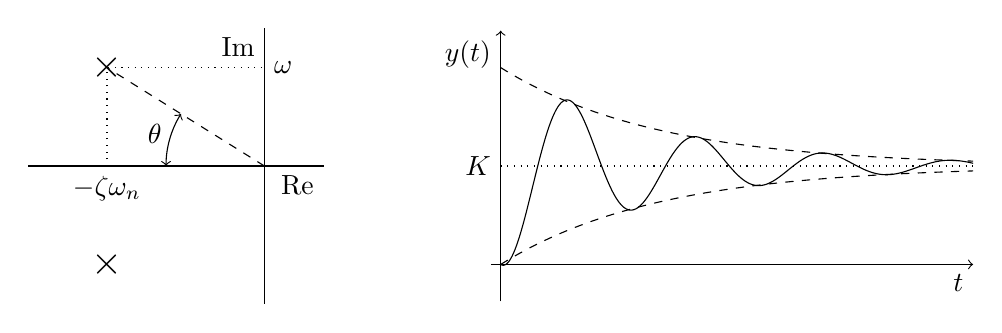
\begin{tikzpicture}
	
	\draw (-3,0) -- (0.75,0) node[below left] {Re};
	\draw (0,-1.75) -- (0,1.75) node[below left] {Im};
	\node at (-2,1.25) {\Large$ \times $};
	\node at (-2,-1.25) {\Large$ \times $};
	\draw[dotted] (-2,0) node[below] {$ -\zeta\omega_n $} |- (0,1.25) node[right] {$ \omega $};
	\draw[dashed] (0,0) -- (-2,1.25);
	\draw[<->] (-1.25,0) arc (180:148:1.25) node[left,pos=0.6] {$ \theta $};
	
	\begin{scope}[shift={(3cm,-1.25cm)},xscale=0.5,yscale=1.25]
		\draw[->] (-0.25,0) -- (12,0) node[below left] {$ t $};  % x Axis
		\draw[->] (0,-0.375) -- (0,2.375) node[below left] {$ y(t) $};  % y Axis
		\draw[domain=0:12,samples=500] plot (\x,{1-(1/sqrt(15))*exp(-\x/4)*( sin(sqrt(15/4)*\x*(180/pi)) + sqrt(15)*cos(sqrt(15/4)*\x*(180/pi))  ) });
		\draw[dotted] (0,1) node[left] {$ K $}-- (12,1);
		\draw[dashed,domain=0:12,samples=500] plot (\x,{1+exp(-\x/4) });
		\draw[dashed,domain=0:12,samples=500] plot (\x,{1-exp(-\x/4) });
	\end{scope}
	
	
	\end{tikzpicture}
\end{center}

%\begin{minipage}{0.37\textwidth}
%	From the pole-zero diagram of $ Y(s) $, it is clear that $ y(t) $ is the sum of a step function and a damped sine (or cosine) wave.
%\end{minipage}
%\begin{minipage}{0.62\textwidth}
%	\begin{center}
%		\begin{tikzpicture}[scale=1]
%		\draw (-2.5,0) -- (1.5,0) node[below left] {Re};
%		\draw (0,-1.75) -- (0,1.75) node[below left] {Im};
%		\node at (-1.5,1) {\Large$ \times $};
%		\node at (-1.5,-1) {\Large$ \times $};
%		\node at (0,0) {\Large$ \times $};
%		\draw (-1.5,0.075) -- (-1.5,0) node[below] {$ -\sigma=-\zeta\omega_n $};
%		\draw (-0.075,1) -- (0,1) node[right] {$ \omega=\omega_n\sqrt{1-\zeta^2} $};
%		\end{tikzpicture}
%	\end{center}
%\end{minipage}
%\begin{align*}
%y(t) &= K_1 + K_2 e^{-\sigma t} \sin (\wt+\phi)\\
%& = A_1 + A_2 e^{-\zeta\omega_n t} \sin \left(\omega_n\sqrt{1-\zeta^2}t+\cos^{-1}\zeta \right)
%\end{align*}
%We already know that
%\[ \lim_{t\to0^+} y(t) = 0,\quad \lim_{t\to0^+} \dot{y}(t) = 0,\quad \lim_{t\to\infty} {y}(t) = K \]
%So, we can roughly sketch
%\begin{center}
%	\begin{tikzpicture}[scale=1.5,xscale=0.5]
%
%	\draw[->] (-0.25,0) -- (12,0) node[below left] {$ t $};  % x Axis
%	\draw[->] (0,-0.5) -- (0,2.5) node[below left] {$ y(t) $};  % y Axis
%	\draw[domain=0:12,samples=500] plot (\x,{1-(1/sqrt(15))*exp(-\x/4)*( sin(sqrt(15/4)*\x*(180/pi)) + sqrt(15)*cos(sqrt(15/4)*\x*(180/pi))  ) });
%	\draw[dotted] (0,1) node[left] {$ K $}-- (12,1);
%	\draw[dashed,domain=0:12,samples=500] plot (\x,{1+exp(-\x/4) });
%	\draw[dashed,domain=0:12,samples=500] plot (\x,{1-exp(-\x/4) });
%
%	\end{tikzpicture}
%\end{center}
%The analytical expression(s) for $ y(t) $ are:
%
%\begin{minipage}{0.49\textwidth}
%	\begin{align*}
%	y(t) &= K \left[1 - \frac{e^{-\sigma t}}{\sin \theta} \sin \left(\wt+\theta\right)\right] \\
%	&= K \left[1 - \frac{e^{-\zw t}}{\sqrt{1-\zeta^2}} \sin \left(\omega_n \sqrt{1-\zeta^2}t+cos^{-1}\zeta\right)\right]
%	\end{align*}
%\end{minipage}
%\begin{minipage}{0.49\textwidth}
%	\begin{center}
%		\begin{tikzpicture}[scale=1.25,yscale=0.8]
%		\draw (-2.5,0) -- (0.5,0) node[below left] {Re};
%		\draw (0,-1.75) -- (0,1.75) node[below left] {Im};
%		\node at (-1.5,1.25) {\Large$ \times $};
%		\node at (-1.5,-1.25) {\Large$ \times $};
%		\draw[dotted] (-1.5,0) node[below] {$ -\sigma $} |- (0,1.25) node[right] {$ \omega $};
%		\draw[dashed] (0,0) -- (-1.5,1.25);
%		\draw[<->] (-1,0) arc (180:140:1) node[left,pos=0.6] {$ \theta $};
%		\end{tikzpicture}
%	\end{center}
%\end{minipage}
The system is said to be \textbf{underdamped}. In this case, damping is not enough to prevent overshoot. Recall that in the overdamped case (real poles), damping is more than enough to prevent overshoot.\\

\textbf{Terminology:}
\begin{itemize}
	\item \textbf{$ \sigma $}: Damping factor
	\item \textbf{$ \zeta $}: Damping ratio
	\item \textbf{$ \omega $} (or $ \omega_d $): Damped natural frequency (the oscillation frequency for $ \sigma\neq0 $ or $ \zeta\neq0 $)
	\item \textbf{$ \omega_n $}: Undamped natural frequency (the oscillation frequency for $ \sigma=\zeta=0 $)
\end{itemize}

Let's now look at some performance characteristics for underdamped second-order systems.
\begin{center}
	\begin{tikzpicture}[scale=2,xscale=0.75,yscale=1.5]
	
	\draw[->] (-0.25,0) -- (10,0) node[below left] {$ t $};  % x Axis
	\draw[->] (0,-0.5) -- (0,2.5) node[below left] {$ y(t) $};  % y Axis
	\draw[domain=0:10,samples=500] plot (\x,{1-(1/sqrt(1-0.1875^2))*exp(-0.1875*2*\x)* sin(  (180/pi)*(2*sqrt(1-0.1875^2)*\x) + acos(0.1875)  ) });
	\draw[dotted] (0,1) node[left] {$ K $}-- (10,1);
	\draw[dashed,domain=0:10,samples=500,color=gray] plot (\x,{1+exp(-\x*2*0.1875) });
	\draw[dashed,domain=0:10,samples=500,color=gray] plot (\x,{1-exp(-\x*2*0.1875) });
	
	\draw[dashed] (0.625,1.55) -| (1.625,0) node[below] {$ t_p $};
	\draw[<->] (0.75,1.55) -- node[left] {$ M_1 $} (0.75,1);
	\draw[<->] (4.875,1) -- node[above] {$ M_2 $} (4.875,1.15);
	
	\draw [dashed] (2.5,1) -- (2.5,0.375);
	\draw [dashed] (5.75,1) -- (5.75,0.375);
	\draw[<->] (5.75,0.45) -- node[below] {Period} (2.5,0.45);
	
	\draw (10,1.04) -- node[above,align=center] {upper tolerance} (8.3125,1.04);
	\draw (10,0.96) -- node[below,align=center] {lower tolerance} (8.3125,0.96);
	\draw[dashed] (8.3125,1.04) -- (8.3125,0) node[below] {$ t_s $};
	
	\draw[dashed] (.9,1) -- (.9,0) node[below] {$ t_r $};
	\end{tikzpicture}
\end{center}
\begin{itemize}
	\item \textbf{Peak Time:} $ t_p = \dfrac{\pi}{\omega} = \dfrac{\pi}{\omega_n\sqrt{1-\zeta^2}} $ This formula is obtained by setting $ dy/dt =0 $. The full derivation can be found in the book on page 175.
	
	Peak time is a measure of how fast the system responds. If you want to decrease the peak time $ t_p $, make $ \omega $ larger, which is done by moving the poles further from the real axis.
	\item \textbf{Percent Overshoot:} $ \%OS = \dfrac{M_1}{K}\times100\% = \dfrac{y_{max}-\lim\limits_{t\to\infty}y(t)}{\lim\limits_{t\to\infty}y(t)}\times100\%$, where $ y_{max} $ is found by evaluating $ y(t) $ at $ t=t_p $. So,
	%%% throughout: get rid of % from 100
	\[ y_{max} = K\left(1+e^{-\frac{\zeta\pi}{\sqrt{1-\zeta^2}}}\right) \]
	Therefore,
	\[ y_{max} - K = M_1 = Ke^{-\frac{\zeta\pi}{\sqrt{1-\zeta^2}}} \quad\Rightarrow\quad \%OS = 100e^{-\pi\zeta / \sqrt{1-\zeta^2}} \]
	The inverse relationship of this is: $ \zeta = \dfrac{-\ln\left(\%OS / 100\right)}{\sqrt{\pi^2+\ln^2\left(\%OS / 100\right)}} $
	
	What does overshoot tell us about peak time? We know that to decrease peak time, we must make $ \omega $ larger. Recall that $ \zeta = \cos \theta $ and note that overshoot increases with decreasing $ \zeta $.
	
	\begin{minipage}{0.49\textwidth}
		\begin{center}
			\begin{tikzpicture}[scale=1.25,yscale=0.8]
			\draw (-2.5,0) -- (0.5,0) node[below left] {Re};
			\draw (0,-1.75) -- (0,1.75) node[below left] {Im};
			\node at (-1.5,1.25) {\Large$ \times $};
			\node at (-1.5,-1.25) {\Large$ \times $};
			\draw[thick,-latex] (-1.5,1.25) -- ++(0,1);
			\draw[thick,-latex] (-1.5,-1.25) -- ++(0,-1);
			\draw[dotted] (0,0) -- (-1.5,1.25+1);
			\draw[dashed] (0,0) -- (-1.5,1.25);
			\draw[<->] (-1,0) arc (180:140:1) node[left,pos=0.6] {$ \theta $};
			\end{tikzpicture}
			
			Moving the poles straight up improves the peak time, but you increase $ \theta $ and therefore increase the overshoot.
		\end{center}
	\end{minipage}
	\begin{minipage}{0.49\textwidth}
		\begin{center}
			\begin{tikzpicture}[scale=1.25,yscale=0.8]
			\draw (-2.5,0) -- (0.5,0) node[below left] {Re};
			\draw (0,-1.75) -- (0,1.75) node[below left] {Im};
			\node at (-1.5,1.25) {\Large$ \times $};
			\node at (-1.5,-1.25) {\Large$ \times $};
			\draw[thick,-latex] (-1.5,1.25) -- ++(-0.75,0.625);
			\draw[thick,-latex] (-1.5,-1.25) -- ++(-0.75,-0.625);
			\draw[dashed] (0,0) -- (-1.5,1.25);
			\node at (-1.5,-2.25) {};
			\draw[<->] (-1,0) arc (180:140:1) node[left,pos=0.6] {$ \theta $};
			\end{tikzpicture}
			
			Moving the poles radially decreases peak time without increasing overshoot.
		\end{center}
	\end{minipage}

	\item \textbf{Time Constant:} $ \tau = \dfrac{1}{\sigma} = \dfrac{1}{\zeta\omega_n} $
	
	The time constant is a measure of the rate of decay of the asymptote, in other words the rapidity at which the exponential term decays, where a larger time constant means it decays slower.
	
	\item \textbf{Settling Time:} $ t_s $ is time to the \textbf{final} entrance to a tolerance band. It is a measure of the duration of the transient response.
	\begin{itemize}
		\item For a $ \pm 5\% $ tolerance band: $ t_s = 3\tau $
		\item For a $ \pm 2\% $ tolerance band: $ t_s = 4\tau $
	\end{itemize}
	Unless specified, settling time typically uses the $ \pm2\% $ tolerance band.

	\item \textbf{Rise Time:} $ t_r $ has multiple definitions; for this course, we will define the rise time as: the time required to go from the initial value (typically 0) to the final value. For this definition, we can construct a mathematical definition of rise time:
	\begin{align*}
	y(t) &= K \left( 1 - \frac{e^{-\zeta\wnt}}{\sin\theta} \sin(\wt+\theta) \right) \\
	&\qquad \text{The final value is $ K $, so look for the first point where $ y(t)=K $:}\\
	K & = K \left( 1 - \frac{e^{-\zeta\wnt_r}}{\sin\theta} \sin(\wt_r+\theta) \right) \\
	1 & = 1 - \frac{e^{-\zeta\wnt_r}}{\sin\theta} \sin(\wt_r+\theta) \\
	0 & = \frac{e^{-\zeta\wnt_r}}{\sin\theta} \sin(\wt_r+\theta) \\
	0 & = \sin(\wt_r+\theta) \\
	\wt_r+\theta & = \pi \\
	\Rightarrow\quad t_r & = \frac{\pi-\theta}{\omega} = \frac{\pi-\theta}{\omega_n\sqrt{1-\zeta^2}}
	\end{align*}
	% (If $ \theta=0 $, this means the rise time is equal to the peak time).
	
	Alternatively, the course book defines rise time as the time required to go from 0.1 (10\%) of the final value to 0.9 (90\%) of the final value. There is no simple analytical relationship between rise time and damping ratio. Typically, it is computed digitally or measured in simulation. Figure 4.16 in the book (page 177) graphically shows a relationship between damping ratio and rise time. 
	
\end{itemize}

\exmp
\[ G(s) = \frac{0.01}{s^2 + 0.002s + 0.01} \]
Our goal is to find: $ \zeta $, $ \omega_n $, $ t_s $, $ t_p $, and $ \%OS $ for a unit step input. To find $ \zeta $ and $ \omega_n $, let's compare $ G(s) $ to the standard form for a 2nd-order transfer function
\[ G(s) = \frac{0.01}{s^2 + 0.002s + 0.01} \Leftrightarrow \frac{K\omega_n^2}{s^2+2\zw s + \omega_n^2} \]
$ G(0) = 1 $ so $ K=1 $. Then,
\[ \omega_n = \sqrt{0.01} = 0.1 \]
\[ 2\zw = 0.002 \quad\Rightarrow\quad \zeta = \frac{0.002}{2\omega_n} = \frac{0.002}{2\cdot0.1} = 0.01 \]
We can now find the performance metrics using $ \omega_n $ and $ \zeta $.
\[ t_p = \frac{\pi}{\omega} = \frac{\pi}{\omega_n\sqrt{1-\zeta^2}} = \frac{\pi}{0.1\sqrt{1-0.01^2}} \approx 31.4 \]
\[ \%OS = 100 e^{\dfrac{-\pi\zeta}{\sqrt{1-\zeta^2}}} = 100e^{\dfrac{-\pi\cdot0.01}{\sqrt{1-0.01^2}}} \approx 96.9\% \]
\[ t_s = 4\tau = \frac{4}{\zeta\omega_n} = \frac{4}{0.01\cdot0.1} = 4000\ sec  \]

\subsection*{Identifying 2nd Order Systems}
How can we re-construct a 2nd-order $ G(s) $ from a time-plot of the step response?

\begin{minipage}{0.4\textwidth}
	\hfill
	\begin{tikzpicture}[scale=1.5,xscale=0.4]		
		\draw[->] (-0.8,0) -- (8,0) node[below left] {$ t $};  % x Axis
		\draw[->] (0,-0.5) -- (0,2.5) node[below left] {$ y(t) $};  % y Axis
		\draw[domain=0:8,samples=500] plot (\x,{1-(1/sqrt(15))*exp(-\x/4)*( sin(sqrt(15/4)*\x*(180/pi)) + sqrt(15)*cos(sqrt(15/4)*\x*(180/pi))  ) });
		\draw[dotted] (0,1) node[left] {}-- (8,1);
	\end{tikzpicture}
\end{minipage}
\begin{minipage}{0.1\textwidth}
	\[ \overset{?}{\Longleftrightarrow} \]
\end{minipage}\begin{minipage}{0.4\textwidth}
	\begin{tikzpicture}[scale=1.25,yscale=0.8]
		\draw (-2.5,0) -- (0.5,0) node[below left] {Re};
		\draw (0,-1.75) -- (0,1.75) node[below left] {Im};
		\node at (-1.5,1.25) {\Large$ \times $};
		\node at (-1.5,-1.25) {\Large$ \times $};
	\end{tikzpicture}
\end{minipage}

\[ G(s)=\frac{K\omega_n^2}{s^2+2\zw s + \omega_n^2} \]
So, we need to find $ K $, $ \omega_n $, and $ \zeta $.
\begin{enumerate}
	\item First, we can find $ K $ from the steady-state value of $ y $:
	\[ K=\lim_{t\to\infty} y(t) \]
	\item Next, we can use the peak time to obtain $ \omega $:
	\[ t_p = \frac{\pi}{\omega} \Rightarrow \omega = \frac{\pi}{t_p} \]
	\item We can get $ \zeta $ from the overshoot percent.
	\[ \%OS = f(\zeta) \Rightarrow \zeta = f^{-1}(\%OS) \]
	Fully written out: 
	\[ \%OS = 100e^{-\pi\zeta / \sqrt{1-\zeta^2}} \quad\Rightarrow\quad \zeta = \dfrac{-\ln\left(\%OS / 100\right)}{\sqrt{\pi^2+\ln^2\left(\%OS / 100\right)}} \]
	\item Finally, using $ \zeta $ and $ \omega $ we can obtain $ \omega_n $
	\[ \omega = \omega_n \sqrt{1-\zeta^2} \Rightarrow \omega_n = \dfrac{\omega}{\sqrt{1-\zeta^2}} \]
\end{enumerate}

\subsection*{Zeros and Higher-Order Systems}
We now have methods for determining the so-called performance specification of a 2nd-order system. That is, we can calculate key characteristics of the system's response to a unit step input. But, all that we have done so far is only valid for a \textbf{2nd order system with no zeros}. Hence, the formulas developed are not valid for a 3rd or 4th order system (for example), nor even for a 2nd order system with a zero.

\paragraph{Question:} Are there circumstances under which these formulas can be used anyways for a higher order system or a for a 2nd order system with a zero? Let's check: Consider a 2nd-order system with a zero at $ s=-\alpha \zeta \omega_n $.

\begin{minipage}{0.4\textwidth}
	\centering
	\[ G(s)=\dfrac{K\frac{\omega_n}{\alpha \zeta}\left(s+\alpha \zeta \omega_n\right)}{s^2+2\zw s + \omega_n^2} \]
	
	(static gain of $ K $)
\end{minipage}
\begin{minipage}{0.4\textwidth}
	\centering
	\begin{tikzpicture}[scale=1.25,yscale=0.8]
		\draw (-3.5,0) -- (0.5,0) node[below left] {Re};
		\draw (0,-1.75) -- (0,1.75) node[below left] {Im};
		\node at (-1.25,1.25) {\Large$ \times $};
		\node at (-1.25,-1.25) {\Large$ \times $};
		\draw (-3,0) node  {\Large$ \circ $} -- ++(0,0) node[below] {$ -\alpha \zeta \omega_n $};
		\draw[<->] (-1.25,-1.0) -- node[above] {$ \zeta\omega $} ++(1.25,0);
	\end{tikzpicture}
\end{minipage}
\begin{align*}
Y(s) &= \frac{1}{s}G(s) \quad\Rightarrow\quad sY(s) = G(s)\\
\lim_{t\to\infty}y(t) & = \lim_{s\to 0}sY(s) = \lim_{s\to 0}G(s) = G(0) = K \\
y(0^+) & = \lim_{s\to\infty}G(s) = \lim_{s\to\infty} \left( K \cdot \dfrac{\dfrac{\omega_n}{\alpha \zeta}\left(\dfrac{1}{s}+\dfrac{\alpha \zeta \omega_n}{s^2}\right)}{1 + \dfrac{2\zw}{s} + \dfrac{\omega_n^2}{s^2}}  \right) = 0\\
\dot{y}(0^+) & = \lim_{s\to\infty} \left[sG(s)\right] \text{   (Note: $ \LT[\dot{y}] = G(s) $)}\\
& = \lim_{s\to\infty} \left( K \cdot \dfrac{\dfrac{\omega_n}{\alpha \zeta}\left(1+\dfrac{\alpha \zeta \omega_n}{s}\right)}{1 + \dfrac{2\zw}{s} + \dfrac{\omega_n^2}{s^2}}  \right) = K \frac{\frac{\omega_n}{\alpha\zeta}}{1} \\
\dot{y}(0^+) & = \frac{K\omega_n}{\alpha\zeta}
\end{align*}
There are two cases for $ \alpha $:
\begin{itemize}
	\item[Case 1:] $ \alpha $ is positive (the zero is in the LHP). Then,
	\begin{itemize}
		\item The initial slope is positive
		\item The system is sped up
		\item Increased overshoot
	\end{itemize} 
	\item[Case 2:] $ \alpha $ is negative (the zero is in the RHP). Then,
	\begin{itemize}
		\item The initial slope is negative (Reverse Action)
		\item The system can be slowed down substantially (high $ t_p $)
		\item Increased overshoot (but not as much as a LHP zero)
		\item Systems with a RHP zero are called ``non-minimum phase'' systems
	\end{itemize} 
\end{itemize}
\begin{center}
	\begin{tikzpicture}[scale=2,xscale=0.875,yscale=1.5]
	
	\draw[->] (-0.5,0) -- (8,0) node[below left] {$ t $};  % x Axis
	\draw[->] (0,-0.5) -- (0,2.5) node[below left] {$ y(t) $};  % y Axis
	\draw[domain=0:8,samples=500] plot (\x,{1-exp(-\x*2*0.1875)*( cos( (180/pi)*sqrt(247/64)*\x ) + (3/sqrt(247))*sin( (180/pi)*sqrt(247/64)*\x)  ) });
	\draw[dotted] (0,1) node[left] {$ K $}-- (8,1);
	
	\draw[dashed,domain=0:8,samples=500] plot (\x,{1-exp(-\x*2*0.1875)*( cos( (180/pi)*sqrt(247/64)*\x ) - (13/sqrt(247))*sin( (180/pi)*sqrt(247/64)*\x)  ) });
	\node[above left] at (1.11,1.82) {$ \alpha>0 $};
	
	\draw[dashed,domain=0:8,samples=500] plot (\x,{1-exp(-\x*2*0.1875)*( cos( (180/pi)*sqrt(247/64)*\x ) + (19/sqrt(247))*sin( (180/pi)*sqrt(247/64)*\x)  ) });
	\node[above right] at (1.96,1.72) {$ \alpha<0 $};
	
	\draw[latex-] (2.3,1.16) -- ++(1,0.4) node[right,align=center] {no zero\\or $ \alpha\to\infty $}; 
	\end{tikzpicture}
\end{center}
If $ \alpha\to\infty $, $ \dot{y}(0^+) \to 0$. So, the extra zero has minimal effect on the output if the zero is far left of the complex poles. How far is necessary? Generally 4 to 5 times as from from the $ \jw $-axis as the complex poles. In other words
\[ \alpha > 4\zeta\omega_n  \text{  or  } \alpha > 5\zeta\omega_n \] 
\begin{center}
	\begin{tikzpicture}[scale=1.25]
	\draw (-7.5,0) -- (0.5,0) node[below left] {Re};
	\draw (0,-1.75) -- (0,1.75) node[below left] {Im};
	\node at (-1.25,1.25) {\Large$ \times $};
	\node at (-1.25,-1.25) {\Large$ \times $};
	\draw (-1.25,0.1) -- (-1.25,0) node[below] {$ \sigma_c $};
	
	\node at (-5.625,0) {\Large$ \circ $};
	\node[below,align=center] at (-5.625,-0.0625) {$ \alpha $};
	\node[below,align=center] at (-5.625,-0.375) {4 to 5 times\\further left};
	
	\end{tikzpicture}
\end{center}

\subsubsection*{3rd and Higher Order Systems}
Third and higher-order systems can be approximated as 2nd-order systems if the extra poles are far left of the dominant complex poles. These extra poles could be either individual real poles or complex conjugate pairs.
\begin{center}
	\begin{tikzpicture}[scale=1.25]
		\draw (-7.5,0) -- (0.5,0) node[below left] {Re};
		\draw (0,-1.75) -- (0,1.75) node[below left] {Im};
		\node at (-1.25,1.25) {\Large$ \times $};
		\node at (-1.25,-1.25) {\Large$ \times $};
		\draw (-1.25,0.1) -- (-1.25,0) node[below] {$ \sigma_c $};
		
		\node at (-5,0) {\Large$ \times $};
		\node at (-6.25,0) {\Large$ \times $};
		\node at (-5.625,0.5) {\Large$ \times $};
		\node at (-5.625,-0.5) {\Large$ \times $};
		
		\draw (-6.5,-.5) arc (180:270:0.25) -- ++(0.375,0) arc (90:0:0.25) node[below,align=center] {4 to 5 times\\further left} arc (180:90:0.25) -- ++(0.375,0) arc (270:360:0.25);
		
	\end{tikzpicture}
\end{center}
We will not go over a derivation for this, but it follows the same method we just used for zeros. In general, if the poles are 4 to 5 times further left of the dominant poles, then the formulas for 2nd-order systems can be used.

\end{document}

